\usepackage{siunitx}


\usetikzlibrary{shadows,shapes.multipart}

\title{Bit Manipulation}


\begin{document}

\begin{frame}
  \titlepage
\end{frame}

\begin{frame}
  \frametitle{Bit Manipulation}
  \begin{itemize}
    \item This topic is not \cpp\ specific
    \item Same is possible in other programming languages
          \begin{itemize}
            \item Often even using exactly the same syntax
          \end{itemize}
  \end{itemize}
\end{frame}

\begin{frame}
  \frametitle{Terminology}
  \begin{itemize}
    \item Rightmost bit is called \emph{least significant bit} (MSB)
    \item Leftmost bit is called \emph{most significant bit} (LSB)
  \end{itemize}
  \begin{overprint}
    \onslide<1|handout:1>
    \structure{\texttt{uint8\_t}}
    \begin{center}
      \begin{tikzpicture}
        \begin{scope}
          \draw (0,0) grid (8,1);
          \foreach[evaluate={\i-0.5} as \x] \i in {1,...,8} {
            \tikzmath{
              int \v;
              \v = random(0, 1);
            }
            \node at (\x, 0.5) {\v};
          }

          \node[anchor=north] (msb) at (0.5,-0.5) {most significant bit};
          \draw[-latex] (msb) -- (0.5,0);

          \node[anchor=north] (lsb) at (7.5,-0.5) {least significant bit};
          \draw[-latex] (lsb) -- (7.5,0);
        \end{scope}
      \end{tikzpicture}
    \end{center}

    \onslide<2|handout:2>
    \structure{\texttt{uint16\_t}}
    \begin{center}
      \begin{tikzpicture}
        \begin{scope}
          \draw (0,0) grid[step=0.5cm] (8,0.5);
          \foreach[evaluate={\i/2-0.25} as \x] \i in {1,...,16} {
            \tikzmath{
              int \v;
              \v = random(0, 1);
            }
            \node[font=\tiny] at (\x, 0.25) {\v};
          }

          \node[anchor=north] (msb) at (0.25,-0.5) {most significant bit};
          \draw[-latex] (msb) -- (0.25,0);

          \node[anchor=north] (lsb) at (7.75,-0.5) {least significant bit};
          \draw[-latex] (lsb) -- (7.75,0);
        \end{scope}
      \end{tikzpicture}
    \end{center}

    \onslide<3|handout:3>
    \structure{\texttt{uint32\_t}}
    \begin{center}
      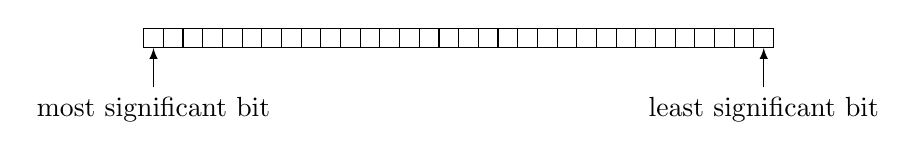
\begin{tikzpicture}
        \begin{scope}
          \draw (0,0) grid[step=0.25cm] (8,0.25);
          \node[anchor=north] (msb) at (0.125,-0.5) {most significant bit};
          \draw[-latex] (msb) -- (0.125,0);

          \node[anchor=north] (lsb) at (7.875,-0.5) {least significant bit};
          \draw[-latex] (lsb) -- (7.875,0);
        \end{scope}
      \end{tikzpicture}
    \end{center}
  \end{overprint}
\end{frame}

\begin{frame}
  \frametitle{Integers}
  \begin{itemize}
    \item \cpp\ offers both signed and unsigned integers
    \item For clarity's sake, examples assume 8-bit integers
    \item But same is applicable on 16, 32, 64, \dots bit integers
  \end{itemize}
\end{frame}

\begin{frame}
  \frametitle{Signed Integers}
  \begin{itemize}
    \item MSB is used to represent sign
    \item If MSB = \texttt{0}, then number is positive ($\geq 0$)
    \item If MSB = \texttt{1}, then number is negative ($< 0$)
    \item Java only offers signed integers
  \end{itemize}
  \begin{center}
    \begin{tikzpicture}[scale=0.75,transform shape]
      \draw (0,0) grid (8,1);
      \foreach[evaluate={\i-0.5} as \x] \i in {1,...,8} {
        \tikzmath{
          int \v;
          \v = random(0, 1);
        }
        \node at (\x, 0.5) {\v};
      }
      \draw[|-|] (0,-0.25) -- (1,-0.25) node[midway,below,font=\tiny] {sign bit};
      \draw[|-|] (1,-0.25) -- (8,-0.25) node[midway,below,font=\tiny] {value};
    \end{tikzpicture}
  \end{center}
  \begin{center}
    \begin{tabular}{ccc}
      \toprule
      \textbf{\# Bits} & \textbf{Lowest} & \textbf{Highest} \\
      \midrule
      8 & $-128$ & $127$ \\
      16 & \num{-32768} & \num{32767} \\
      32 & $-2^{31}$ & $2^{31}-1$ \\
      64 & $-2^{63}$ & $2^{63}-1$ \\
      $N$ & $-2^{N-1}$ & $2^{N-1}-1$ \\
      \bottomrule
    \end{tabular}
  \end{center}
\end{frame}

\begin{frame}
  \frametitle{Unsigned Integers}
  \begin{itemize}
    \item All bits are used to represent value
  \end{itemize}
  \begin{center}
    \begin{tikzpicture}[scale=0.75,transform shape]
      \draw (0,0) grid (8,1);
      \foreach[evaluate={\i-0.5} as \x] \i in {1,...,8} {
        \tikzmath{
          int \v;
          \v = random(0, 1);
        }
        \node at (\x, 0.5) {\v};
      }
      \draw[|-|] (0,-0.25) -- (8,-0.25) node[midway,below,font=\tiny] {value};
    \end{tikzpicture}
  \end{center}
  \begin{center}
    \begin{tabular}{ccc}
      \toprule
      \textbf{\# Bits} & \textbf{Lowest} & \textbf{Highest} \\
      \midrule
      8 & $0$ & $255$ \\
      16 & \num{0} & \num{65535} \\
      32 & $0$ & $2^{32}-1$ \\
      64 & $0$ & $2^{64}-1$ \\
      $N$ & $0$ & $2^{N}-1$ \\
      \bottomrule
    \end{tabular}
  \end{center}
\end{frame}

\end{document}
